\documentclass[a4paper,12pt]{article}
\usepackage[utf8]{inputenc}
\usepackage[spanish]{babel}
\usepackage{color}
\usepackage{parskip}
\usepackage{graphicx}
\usepackage{multirow}
\usepackage{listings}
\usepackage{vmargin}
\graphicspath{ {imagenes/} }
\definecolor{mygreen}{rgb}{0,0.6,0}
\definecolor{lbcolor}{rgb}{0.9,0.9,0.9}
\usepackage{epstopdf}


\setpapersize{A4}
\setmargins{2.5cm}       % margen izquierdo
{1.5cm}                        % margen superior
{16.5cm}                      % anchura del texto
{23.42cm}                    % altura del texto
{10pt}                           % altura de los encabezados
{1cm}                           % espacio entre el texto y los encabezados
{0pt}                             % altura del pie de página
{2cm}     

\lstset{
    tabsize=4,    
%   rulecolor=,
    language=[GNU]C++,
        basicstyle=\tiny,
        aboveskip={1.5\baselineskip},
        columns=fixed,
        showstringspaces=false,
        extendedchars=false,
        breaklines=true,
        prebreak = \raisebox{0ex}[0ex][0ex]{\ensuremath{\hookleftarrow}},
        frame=single,
        showtabs=false,
        showspaces=false,
        showstringspaces=false,
        identifierstyle=\ttfamily,
        keywordstyle=\color[rgb]{0,0,1},
        commentstyle=\color[rgb]{0.026,0.112,0.095},
        stringstyle=\color{red},
        numberstyle=\color[rgb]{0.205, 0.142, 0.73},
%        \lstdefinestyle{C++}{language=C++,style=numbers}’.
}

\begin{document}
\begin{titlepage}

\begin{center}
\vspace*{-1in}

\begin{large}
UNIVERSIDAD NACIONAL DE SAN AGUSTÍN\\
\vspace*{0.15in}
ESCUELA PROFESIONAL DE CIENCIA DE LA COMPUTACIÓN\\
\end{large}
\begin{figure}[htb]
\centering

\includegraphics[scale=0.13]{/home/xnpio/Documentos/Caratula/logo.eps}
\end{figure}
\vspace*{0.15in}
\begin{large}
TEMA:\\
\end{large}
\vspace*{0.2in}
\begin{Large}
\textbf{MÉTODO DE LAS POTENCIAS EN FORTRAN} \\
\end{Large}
\vspace{8mm}

\begin{large}
Curso:\\
\end{large}
\vspace*{0.2in}
\begin{Large}
\textbf{MATEMÁTICA APLICADA A LA COMPUTACIÓN} \\
\end{Large}

\vspace{8mm}

\begin{large}
\textbf{Presentado por:}\\

\begin{flushleft}

\hspace{7cm} Christofer Chávez Carazas \\

\end{flushleft}
\end{large}
\vspace{4cm}
\rule{80mm}{0.1mm}\\
\vspace*{0.1in}

\begin{large}
Arequipa - Perú \\
2017 \\
\end{large}
\end{center}
\end{titlepage}

\twocolumn[]
  \section{Código}
  \begin{lstlisting}
program potencias

	integer :: i = 0
	integer :: j = 0
	integer :: m = 2
	integer :: n = 2
	real(16), dimension(3,3) :: matrix
	real(16), dimension(3) :: ini

	matrix(1,1) = 3
	matrix(1,2) = -1
	matrix(1,3) = 0

	matrix(2,1) = -1
	matrix(2,2) = 2
	matrix(2,3) = -1

	matrix(3,1) = 0
	matrix(3,2) = -1
	matrix(3,3) = 3

	ini(1) = 1
	ini(2) = 1
	ini(3) = 1

	call Mpotencias(matrix,ini,3,10)

	

end program	potencias

subroutine Mpotencias(M,ini,N,iter)
	integer :: i = 0
	real(16), dimension(N,N) :: M
	real(16), dimension(N) :: v
	real(16), dimension(N) :: u
	real(16), dimension(N) :: ini
	real(16) :: dominante,temp
	v = ini
	do i = 1,iter
		call mul(M,v,N,u)
		call mayor(u,N,dominante)
		temp = 1.0 / dominante
		call mulnum(u,temp,N,v)
		call printMatriz(u,N,1)
		write(*,*)
		call printMatriz(v,N,1)
		write(*,*)
	end do

return
end subroutine Mpotencias

subroutine mayor(M,N,res)
	real(16), dimension(N) :: M
	real(16) :: res,temp
	integer :: i
	res = -1
	do i = 1,N
		temp = abs(M(i))
		if((res == -1) .or. (res < temp)) then
			res = temp
		end if
	end do
return
end subroutine mayor

subroutine printMatriz(M,f,c)
	integer :: i,j
	integer :: f,c
	real(16), dimension(f,c) :: M
	do i=1,f
    	do j=1,c
        	write(*,'(F10.6,$)') M(i,j)
    	end do
    	write(*,*)
	end do
return
end subroutine printMatriz


subroutine mul(A,B,N,res)
	integer :: N,i,j,k
	real(16), dimension(N,N) :: A
	real(16), dimension(N) :: B
	real(16), dimension(N) :: res
	real(16) :: sum

	do i=1,N
		sum = 0
		do j=1,N
			sum = sum + B(j) * A(i,j)
		end do
		res(i) = sum
	end do
return
end subroutine mul

subroutine mulnum(A,x,N,res)
	integer :: N,i
	real(16) :: x
	real(16), dimension(N) :: A,res
	do i=1,N
		res(i) = A(i) * x
	end do
return
end subroutine mulnum

  \end{lstlisting}
\section{Ejemplo}

La matriz usada en este ejemplo es la siguiente:

\[ A = \left[ \begin{array}{ccc}
3 & -1 & 0 \\
-1 & 2 & -1 \\
0 & -1 & 3 \end{array} \right]\]

\textbf{Número de iteraciones: } $5$

\onecolumn

\section{Resultados}

Se imprime primero la matriz $u$ y luego la matriz $v$ en cada iteración.

\begin{figure}[h]
 \centering
 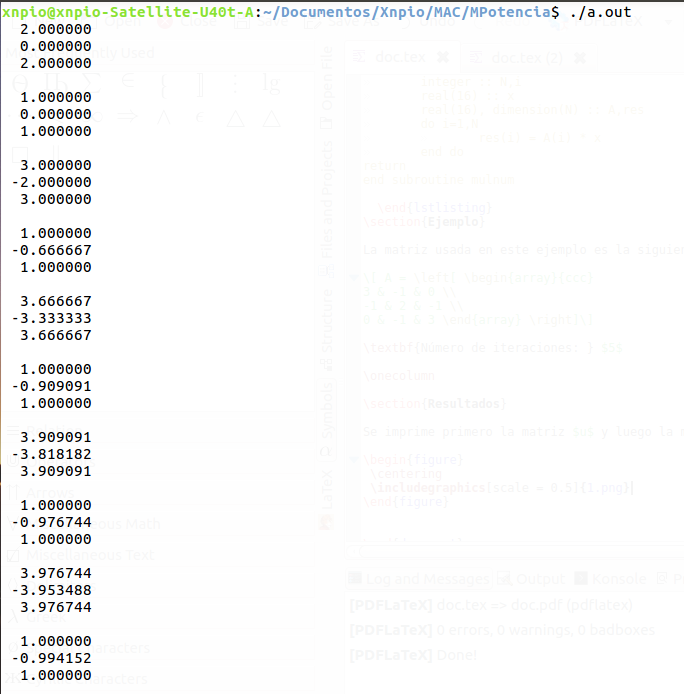
\includegraphics[scale = 0.5]{1.png}
\end{figure}


\end{document}
